\section{Problemas propuestos}

\begin{section-problem}
    Sea $D$ el pie de altura desde $A$ en el triángulo \theTriangle{ABC} y $M$, $N$ puntos en los lados $CA$ y $AB$ talque las rectas $BM$ y $CN$ se intersecan en $AD$.
    Probar que $AD$ es bisectriz del ángulo $\angle MDN$.
\end{section-problem}

\begin{hint}
    Sea $T$ la intersección de $AD$ y $MN$, probar que $\frac{TM}{TN} = \frac{DM}{DN}$.
    Considerar aplicar el teorema de la bisectriz generalizada al triángulo \theTriangle{ABC} y La ley de los senos a los triángulos \theTriangle{BDN} y \theTriangle{CDM}.
    Utilizar la propiedad $\sin(90^\circ - \alpha) = \cos(\alpha)$ y luego probar que $\tan(\angle MDA) = \tan(\angle NDA)$.
\end{hint}

\begin{solution}
    \begin{figure}[H]
        \centering
        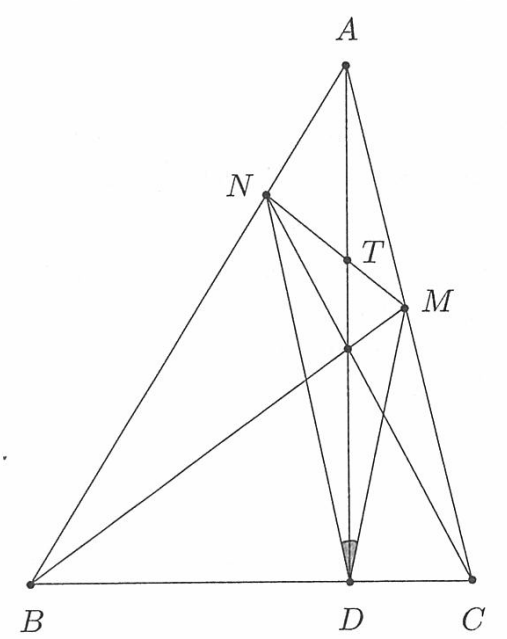
\includegraphics[width=7cm]{images/p1}
        \caption{Problema 1.}
    \end{figure}
    Sea $T$ la intersección de $AD$ con $MN$.
    Por el teorema de la bisectriz generalizada, tenemos que
    \[
        \frac{TM}{TN} = \frac{AM}{AN}\cdot \frac{\sin{(DAC)}}{\sin{(DAB)}}.
    \]
    También, por el teorema de la bisectriz generaliza, podemos decir que
    \[
        \frac{DC}{DB} = \frac{AC}{AB} \cdot \frac{\sin{(DAC)}}{\sin{(DAB)}}.
    \]
    Por consiguiente, tenemos que
    \[
        \frac{TM}{TN} = \frac{AM}{AN}\cdot \frac{DC}{DB}\cdot \frac{AB}{AC} = \frac{AM}{AN}\cdot \frac{DC}{DB}\cdot \frac{\sin{(C)}}{\sin{(B)}},
    \]
    donde la última ecuación se deduce por la ley de lo Senos aplicado al triángulo \theTriangle{ABC}.
    Por otro lado, por la misma ley de los Senos, aplicada a los triángulos \theTriangle{BDN} y \theTriangle{CDM}, temos que
    \[
        DM = CM \cdot \frac{\sin{(C)}}{\sin{(CDM)}} = CM \cdot \frac{\sin{(C)}}{\sin{(90^{\circ} - MDA)}} = CM \cdot \frac{\sin{(C)}}{\cos{(MDA)}},
    \]
    y análogamente
    \[
        DN = BN \cdot \frac{\sin{(B)}}{\cos{NDA}};
    \]
    entonces,
    \[
        \frac{DM}{DN} = \frac{CM}{BN} \cdot \frac{\sin{(C)}}{\sin{(B)}} \cdot \frac{\cos{(NDA)}}{\cos{(MDA)}}.
    \]    
    Pero las rectas $AD, BM, CN$ son concurrentes, por lo que por el teorema de Ceva sabemos que
    \[
        \frac{DB}{DC}\cdot \frac{MC}{MA}\cdot \frac{NA}{NB} = 1,\ \text{es decir}\ \frac{DC}{DB} \cdot \frac{AM}{AN} = \frac{CM}{BN}.
    \]
    Por consiguiente, tenemos que
    \[
        \frac{TM}{TN} = \frac{CM}{BN} \cdot \frac{\sin{(C)}}{\sin{(B)}} = \frac{DM}{DN} \cdot \frac{\cos{(MDA)}}{\cos{(NDA)}}.
    \]
    Pero, por el teorema de la bisectriz generalizada nos da que
    \[
        \frac{TM}{TN} = \frac{DM}{DN} \cdot \frac{\sin{(MDA)}}{\sin{(NDA)}};
    \]
    de este modo $\tan{(MDA)} = \tan{(NDA)}$, y entonces los angulos $\angle MDA = \angle NDA$ son iguales, como se afirma.
\end{solution}


\begin{section-problem}
    Sea \theTriangle{ABC} un triángulo con incentro $I$.
    Sea $\Gamma$ un círculo centrado en $I$ con radio mayor al inradio.
    Sean $X_1$ la intersección de $\Gamma$ con $AB$ más cercana a $B$; $X_2$ y $X_3$ las intersecciones de $\Gamma$ con $BC$ donde $X_2$ es más cercana a $B$; y $X_4$ la intersección de $\Gamma$ con $CA$ más cercana a $C$.
    Sea $K$ la intersección de $X_1 X_2$ con $X_3 X_4$.
    Probar que $AK$ biseca $X_2 X_3$.
\end{section-problem}

\begin{hint}
    Sean $D, E$ y $F$ a los puntos de tangecias del incírculo con $BC, CA$ y $AB$, respectivamente.
    Demuestra que $FX_1 = DX_2 = EX_4$.
\end{hint}

\begin{solution}
    Sean $D, E$ y $F$ los puntos de tangencia del incírculo con $BC, CA$ y $AB$, respectivamente.

    Por Pitágoras $X_2 D = \sqrt {X_2 I^2 - ID^2} = \sqrt {X_1 I^2 - IF^2} = X_1 F$, y como $BF = BD$, entoncees $BX_1 = BX_2$.
    De este modo $X_1 X_2 || DE$, y de manera análoga $X_3 X_4 || DE$ y $FE || X_1 X_4$.

    Por lo tanto los triángulos \theTriangle{DEF} y \theTriangle{X_1 X_4 K} son homotéticos y las rectas $X_1 F$, $X_4 E$ y $KD$ concurren en $A$, y dado que $D$ es el punto medio de $X_2 X_3$ se demuestra el resultado pedido.
\end{solution}


\begin{section-problem}
    Sea $ABCD$ un cuadrado y sea $X$ un punto en lado $BC$.
    Sea $Y$ un punto en la recta $CD$ tal que $BX = YD$ y $D$ se encuentra entre $C$ y $Y$.
    Demuestra que el punto medio de $XY$ se encuetra sobre la diagonal $BD$.
\end{section-problem}

\begin{hint}
    Aplicar el teorema de Menelao a los triángulos \theTriangle{BCD} y \theTriangle{XCY}.
\end{hint}


\begin{section-problem}
    Sean $\Gamma_1$ una circunferencia y $P$ un punto fuera de $\Gamma_1$.
    Las rectas tangentes desde $P$ a $\Gamma_1$ tocan a la circunferencia en los puntos $A$ y $B$.
    Considera $M$ el punto medio del segmento $PA$ y $\Gamma_2$ la circunferencia que pasa por los puntos $P, A$ y $B$.
    La recta $BM$ interseca de nuevo a $\Gamma_2$ en el punto $C$, la recta $CA$ interseca de nuevo a $\Gamma_1$ en el punto $D$, el segmento $DB$ interseca de nuevo a $\Gamma_2$ en el punto $E$ y la recta $PE$ interseca a $\Gamma_1$ en el punto $F$ (con $E$ entre $P$ y $F$).
    Muetra que las rectas $AF, BP$ y $CE$ concurren.
\end{section-problem}

\begin{hint}[\textbf{Olimpiada Mexicana de Matemáticas, 2014}]
    Probar que los triángulos \theTriangle{BEF} y \theTriangle{PCA} son homotéticos.
\end{hint}

\begin{figure}[H]
    \centering
    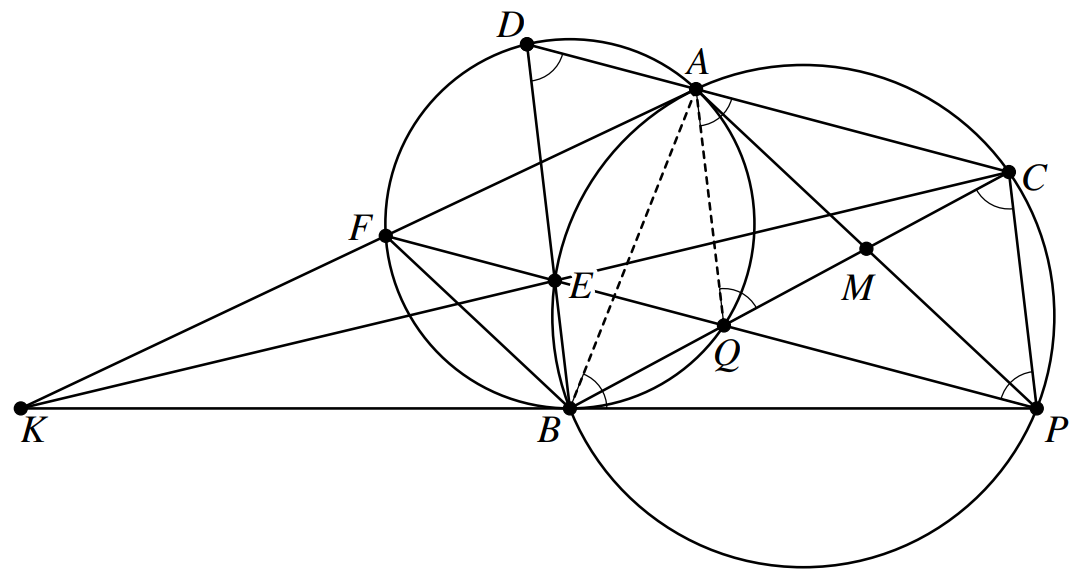
\includegraphics[width=12cm]{images/p3}
    \caption{Problema 3.}
\end{figure}

\begin{solution}
    Sea $Q$ el segundo punto de intersección de $BC$ y $\Gamma_1$.
    Como $MA$ es tangente a $\Gamma_1$, notemos que
    \[
        MQ \cdot MB = MA^2 = MA \cdot MP = MC \cdot MB
    \]
    así que $M$ también es punto medio de $CQ$.
    Siendo así, $AQPC$ un paralelogramo.
    Luego, conseguimos
    \[
        \angle CQA = \angle QCP = \angle BCP = \angle BAP = \angle PBA = 180^{\circ} - \angle ACP = \angle QAC
    \]
    de modo que $QCA$ es isósceles en $A$, por lo que $AQBD$ es un trapecio isóscels.
    Esto se traduce en $BE || QA || PC$.
    Además, $\angle BEP = \angle BPC = \angle QAC = \angle BDC$, por tanto $QE || AD$, así que forzosamente $P, Q$ y $E$ están alineados.
    Tomando en cuenta la definición de $F$, podemos inferir que $EF || CA$ y que $AQFD$ es un trapecio isósceles.
    Esto conlleva a que $\angle BFQ = \angle BAQ = \angle PAC = \angle QPA$, luego $BF || PA$.

    En resumen, los lados correspondientes de \theTriangle{BEF} y \theTriangle{PCA} son paralelos, por lo que estos triángulos son homotéticos; por consiguiente, $AF, CE$ y $PB$ concurren en el centro de homotecia de estos triángulos.
\end{solution}


\begin{section-problem}
    Sea $\Omega$ el circuncírculo del triángulo \theTriangle{ABC} y sea $\omega_a$ la circunferencia tangente al segmento $CA$, segmento $AB$ y $\Omega$.
    Se definen $\omega_b$ y $\omega_c$ de manera análoga.
    Sea $A', B', C'$ los puntos de toque de $\omega_a, \omega_b, \omega_c$ con $\Omega$, respectivamente.
    Probar que $AA', BB', CC'$ concurren en la recta $OI$ donde $O$ e $I$ son el cincuncentro y el incentro de \theTriangle{ABC}, respectivamente.
\end{section-problem}

\begin{hint}
    Considerar el incírculo del triángulo \theTriangle{ABC} y considerar el exsimilicentro de este con $\Omega$.
    Luego, aplicar los teoremas de Monge y Monge D'Alembert.
\end{hint}


\begin{section-problem}
    Sea $ABCD$ un trapezoide con $AB > CD$ y $AB || CD$.
    Sean los puntos $K, L$ sobre los segmentos $AB, CD$, respectivamente, tal que $\frac{AK}{KB} = \frac{DL}{LC}$.
    Suponga que existen los puntos $P, Q$ en la recta $KL$ que satisfacen $\angle APB = \angle BCD$ y $\angle CQD = \angle ABC$.
    Probar que los puntos $P, Q, B, C$ con concíclicos.
\end{section-problem}

\begin{hint}
    Considerar la intersección de $AD$ con $BC$ y analizar si existe alguno homotecia centrado en ese punto.
    Luego, por medio de angulo en cuadrilátero cíclicos llegar a lo pedido.
\end{hint}



\begin{section-problem}
    Los puntos $P$, $Q$ y $R$ están sobre los lados $AB$, $BC$ y $CA$ del triángulo acutángulo \theTriangle{ABC}, respectivamente.
    Si $\angle BAQ = \angle CAQ$, $QP \perp AB$, $QR \perp AC$ y $CP$ y $BR$ se intersecan en $S$ probar que $AS \perp BC$.
\end{section-problem}

\begin{hint}
    Aplicar Ceva al triángulo \theTriangle{ABC} con los puntos $P$, $Q$ y $R$.
    Utilizar la definición del coseno.
\end{hint}



\begin{section-problem}
    Sea \theTriangle{ABC} un triángulo con circuncentro $O$ y baricentro $G$.
    Sean $A', B', C'$ las reflexiones de los puntos medios de $BC, CA, AB$ con respecto a $O$, respectivamente.
    Probar que $AA', BB', CC'$ y $GO$ con concurrente.
\end{section-problem}

\begin{hint}
    Considere el ortocentro $H$, y demuestre que los triángulos \theTriangle{ABH} y \theTriangle{A'B'O} son homotéticos.
\end{hint}


\begin{section-problem}
    Un triángulo isósceles \theTriangle{ABC} tiene base $AB$ y altura $CD$ con $BC = CA$.
    Sean $P$ un punto sobre $CD$, $E$ la intersección de la recta $AP$ con $BC$ y $F$ la intersección de la recta $BP$ con $CA$.
    Suponga que los incírculos del triángulo \theTriangle{ABP} y del cuadrilátero $PECF$ son congruentes.
    Demuestre que los incírculos de \theTriangle{ADP} y \theTriangle{BCP} son también congruentes.
\end{section-problem}

\begin{hint}
    Trazar la tangente común externa más cercana al punto $A$, y note que esta es paralela a $CD$.
    Considera ahora una homotecia de centro $B$.
\end{hint}


\begin{section-problem}
    Sea el triángulo \theTriangle{ABC} con $AC = BC$, sea $P$ un punto dentro del triángulo tal que $\angle PAB = \angle PBC$.
    Si $M$ es el punto medio de $AB$, entonce probar que $\angle APM + \angle BPC = 180^{\circ}$.
\end{section-problem}

\begin{hint}
    Probar que $CA$ y $CB$ son tangentes a circuncírculo del triángulo \theTriangle{APB}.
    Luego, usar la construción de simediana.
\end{hint}



\begin{section-problem}
    Sea $P$ un punto en el plano del triángulo \theTriangle{ABC} y sea $Q$ su conjugado isogonal respecto a \theTriangle{ABC}.
    Probar que
    \[
        \frac{AP \cdot AQ}{AB \cdot AC} + \frac{BP \cdot BQ}{BA \cdot BC} + \frac{CP \cdot CQ}{CA \cdot CB} = 1.
    \]
\end{section-problem}

\begin{hint}[Lista corta, IMO 1998]
    Considerar a $X, Y, Z$ los pies de las proyecciones desde $P$ hacía $BC, CA, AB$, respectivamente.
    Luego, utilizar áreas para lograr el resultado.
\end{hint}


\begin{section-problem}
    Sea el triángulo \theTriangle{ABC} y $P$ un punto en su interior.
    Sea $A_1$, $B_1$ y $C_1$ las intersecciones de $AP$, $BP$ y $CP$ con los lados $BC$, $CA$ y $AB$, respectivamente.
    Considerando a $X$, $Y$ y $Z$ como la intersecciones de $BC$ con $B_1 C_1$, $CA$ con $C_1 A_1$ y $AB$ con $A_1 B_1$, respectivamente.
    Probar que $X$, $Y$ y $Z$ son colineales.
\end{section-problem}

\begin{hint}
    Aplicar Menelao al triángulo \theTriangle{ABC} tres veces y multiplicar los resultados.
\end{hint}


\begin{section-problem}
    Sea el triángulo \theTriangle{ABC} con incentro $I$.
    Sean $D, E, F$ puntos de tangecias de su circuncírculo con los lados $BC$, $CA$ y $AB$, respectivamente.
    Probar que los circuncírculos de los triángulos \theTriangle{AID}, \theTriangle{BIE} y \theTriangle{CIF} tiene dos puntos en común.
\end{section-problem}

\begin{hint}
    Probar que los centros de los círculos son colineales.
    Sean $O_1, O_2, O_3$ lo centros de los circuncírculos de los triángulos en cuestión, considerar la reflexión de $I$ con respecto a estos centros.
\end{hint}


\begin{section-problem}
    Sea $BCXY$ un rectángulo construido fuera del triángulo \theTriangle{ABC}.
    Sea $D$ pie de altura desde $A$ hacía $BC$ y sean $U$ y $V$ los puntos de intersección de $DY$ con $AB$ y $DX$ con $AC$, respectivamente.
    Probar que $UV || BC$.
\end{section-problem}

\begin{hint}
    Aplicar el teorema de Desargues en una de sus versiones degeneradas.
\end{hint}

\begin{section-problem}
    Sea el triángulo \theTriangle{ABC} con $AB < AC$, el punto $H$ denota el ortocentro.
    Los puntos $A_1$ y $B_1$ son pies de alturas desde $A$ y $B$, respectivamente.
    El punto $D$ es la reflexión de $C$ respecto al punto $A_1$.
    Si $E = AC \cap DH$, $F = DH \cap A_1 B_1$ y $G = AF \cap BH$, probar que las rectas $CH$, $EG$ y $AD$ concurren.
\end{section-problem}

\begin{hint}
    Aplicar el teorema de Desargues.
\end{hint}


\begin{section-problem}
    Las circunferencias $C_1$ y $C_2$ son tangentes externamente.
    Las rectas tangentes desde $O_1$ hacia $C_2$ la tocan en $A$ y $B$; mientras que las rectas tangentes desde $O_2$ hacia $C_1$ la tocan en $C$ y $D$, respectivamente.
    Sean $E = O_1 A \cap O_2 C$ y $F = O_1 B \cap O_2 D$.
    Demostrar que $EF$, $O_1 O_2$, $AD$ y $BC$ concurren.
\end{section-problem}

\begin{hint}
    Aplicar el teorema de Pascal.
\end{hint}

\begin{section-problem}
    Sea el triángulo \theTriangle{ABC}, y sean los puntos $B_1$, $C_1$ sobre los lados $CA$ y $AB$ respectivamente.
    Sea $\Gamma$ el incírculo del \theTriangle{ABC} y sean $E$ y $F$ los puntos de tangencias de $\Gamma$ con los mismos lados $CA$ y $AB$, respectivamente.
    Además, se dibujan las tangentes desde $B_1$ y $C_1$ a \theTriangle{ABC} y se toma los puntos de tangecias $Z$ y $Y$, respectivamente.
    Probar que las rectas $B_1 C_1$, $EF$ y $YZ$ son concurrentes.
\end{section-problem}

\begin{hint}
    Aplicar el teorema de Pascal en dos hexágonos degenerados.
\end{hint}


\begin{section-problem}
    Sea el triángulo \theTriangle{ABC} y sea $P$ un punto en el interior del triángulo pedal \theTriangle{DEF}.
    Suponga que las rectas $DE$ y $DF$ son perpendiculares.
    Probar que si $Q$ es el conjugado isogonal de $P$ con respecto al triángulo \theTriangle{ABC}, entonces $Q$ es el ortocentro del triángulo \theTriangle{AEF}.
\end{section-problem}

\begin{hint}
    Considerar las reflexiones $A', B', C'$ de $P$ con respecto a $BC, CA, AB$, respectivamente.
    Luego, probar que $Q$ es punto medio de $B'C'$.
\end{hint}


\begin{section-problem}
    Sea \theTriangle{ABC} un triángulo cualquiera y $D$, $E$ y $F$ puntos cualesquiera sobre las rectas $BC$, $CA$ y $AB$ tal que las rectas $AD$, $BE$ y $CF$ concurren.
    La paralela a $AB$ por $E$ interseca a la recta $DF$ en el punto $Q$, la paralela a $AB$ por $D$ interseca a $EF$ en $T$.
    Probar que la rectas $CF$, $DE$ y $QT$ son concurrentes.
\end{section-problem}

\begin{hint}
    Por conveniencia, considerar dibujar los puntos $D, E, F$ en el interior de los segmentos $BC, CA, AB$.
    Aplicar varias veces el teorema de Ceva y el teorema de la bisectriz generalizada.
\end{hint}


\begin{section-problem}
    El punto $D$ está sobre el lado $AB$ del triángulo \theTriangle{ABC}.
    Sea $\omega_1$ y $\Omega_1$, $\omega_2$ y $\Omega_2$ los incírculos y los excírculos (tangentes al segmento $AB$) de los triángulos \theTriangle{ACD} y \theTriangle{BCD}, respectivamente.
    Probar que las tangentes externas comunes a $\omega_1$ y $\omega_2$, $\Omega_1$ y $\Omega_2$ se intersecan en $AB$.
\end{section-problem}

\begin{hint}
    Considerar los centro de los círculos en cuestión y luego aplicar el teorema de Desargues.
\end{hint}


Nota: los problemas no están ordenados por orden de dificultad.